% Inherently colored legacy patterns.
\usetikzlibrary{patterns}

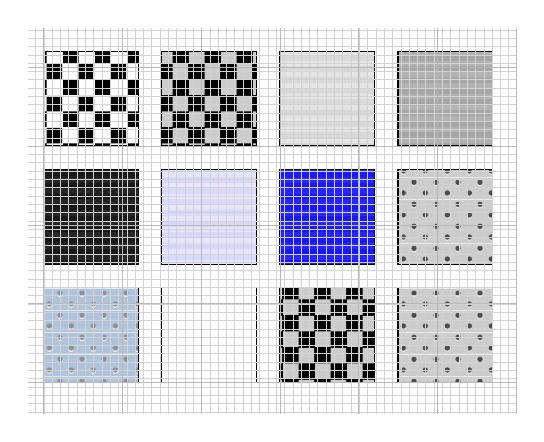
\begin{tikzpicture}[x=1cm,y=1cm]
  \path[draw,pattern=checkerboard] (0,0) rectangle +(1.2,1.2);
  \path[draw,pattern=checkerboard light gray] (1.5,0) rectangle +(1.2,1.2);
  \path[draw,pattern=horizontal lines light gray] (3.0,0) rectangle +(1.2,1.2);
  \path[draw,pattern=horizontal lines gray] (4.5,0) rectangle +(1.2,1.2);

  \path[draw,pattern=horizontal lines dark gray] (0,-1.5) rectangle +(1.2,1.2);
  \path[draw,pattern=horizontal lines light blue] (1.5,-1.5) rectangle +(1.2,1.2);
  \path[draw,pattern=horizontal lines dark blue] (3.0,-1.5) rectangle +(1.2,1.2);
  \path[draw,pattern=crosshatch dots gray] (4.5,-1.5) rectangle +(1.2,1.2);

  \path[draw,pattern=crosshatch dots light steel blue] (0,-3.0) rectangle +(1.2,1.2);
  \path[draw,fill=yellow!50,pattern=none] (1.5,-3.0) rectangle +(1.2,1.2);
  \path[draw,pattern=checkerboard light gray,pattern color=red] (3.0,-3.0) rectangle +(1.2,1.2);
  \path[draw,pattern=crosshatch dots gray,pattern color=blue] (4.5,-3.0) rectangle +(1.2,1.2);

  % Overlay reference grid for easier phase/offset comparison.
  \draw[step=3pt,gray!35,line width=.1pt] (-0.2,-3.4) grid (6.0,1.5);
  \draw[step=1cm,gray!55,line width=.16pt] (-0.2,-3.4) grid (6.0,1.5);
\end{tikzpicture}
